\chapter{Methodology}
\label{chap:methodology}


\section{Tool}
The goals 
\section{Electromagnetic exposure}
\subsection{Calculation of total whole body SAR10g} % (fold)
\label{sub:Calculationexposure}

The overall $SAR^{head}_{10g}$ can be calculated by a simple sum of individual SAR values \cite{J17_kuehn2019modelling}. 
The position of the phone is however unknown. This is because the tool assigns a bitrate to a user depending on the service he is using
meaning that users in the network are not only calling but are able of browsing the web aswell. 
Since calculating the $SAR^{head}_{10g}$ would imply the phone is being hold next to the head, this would result in incorrect conclusions.
The induced electromagnetic radiation will therefore be expressed in function of the entire body.


\begin{equation} 
SAR^{wb,total}_{10g} = SAR^{wb,ul}_{10g} +  SAR^{wb,dl}_{10g} + SAR^{wb,neighbours}_{10g}
\label{eq:overallSARwb}
\end{equation}

The first parameter, $SAR^{wb,ul}_{10g}$, will indicate the absorbed electromagnetic radiation in the whole body originating from the users own phone
whereas the second parameter $SAR^{wb,dl}_{10g}$ will represent the absorbed electromagnetic radiation by all the basestations in the considered area.
As last, $SAR^{wb,neighbours}_{10g} $ specifies the same as the previous but with electromagnetic radiation originating from other users their \gls{UE}.

\subsection{Calculating downlink expsure} % (fold)
\label{sub:Calculating downlink expsure}

\subsubsection{Calculating exposure towards a single femtocell}
\label{sec:calculatingexposure}

To determine the total exposure of a single human being or even of the entire network, the electric-field $\vec{E}$ of a single femtocell $i$ should be calculated.
The formula to determine this electromagnetic value $E$ (expressed in V/m) for a specific location is given in equation \ref{eq:singleexposure}.
\begin{equation}
E_i = 10^{\frac{EIRP - 43.15 + 20*\log(f)- PL}{20}}
\label{eq:singleexposure}
\end{equation}
TODO: write EIRP - Attenuation (A t)\\
This formula requires several values to be known. The frequency $f$ on which the tranmitting antenna is operating is expressed in MHz. The other values are explained in \ref{subsec:eirp} and \ref{subsec:pl}.
\paragraph{Equivalent Isotropical Radiation Power}
\label{subsec:eirp}

A directional antenna can achieve gain by focussing it's input power into certain directions. By doing this, some areas experience a decreased radiation power in order to gain radiation power 
in the other privileged areas. If a theorical isotropic radiator \color{red}todo: uileggen wat isotropic radiator is\color{black} existed, the \gls{EIRP} is the power it would require to achieve the same power level as the actual antenna's main lob. The main lob is the area of the directional antenna experiencing the most gain.
This \gls{EIRP} value can be calulated as described in eq \ref{eq:eirp}.
\begin{equation}
EIRP = P_t + G_t - L_t
\label{eq:eirp}
\end{equation}

\paragraph{Pathloss}
\label{subsec:pl}
At last, formula \ref{eq:eirp} requires the path loss (dB). In order calculate the path loss, an appropiate propagation model is required. Several propagation models exists and the tool already uses the Walfish-Ikegami model \cite{J2}.
This is because the Walfish-Ikegami model performs well for femtocell networks in urban areas. %optioneel kan je hier dezelfde bron gebruiken als dat ze in thesis van de vorige gebruikten. Bron nummer 32
The chosen propagation model consists of two formulas depending on whether a free line of sight between the user and the basestation exist or not. Both formulas expect a distance in kilometer. %bron?

input power hangt af van bs tot bs.
\paragraph{Attenuation}
todo

\subsubsection{Combining exposure}
\label{sec:combiningexposure}
Since the user location in the UAV-aided network is known, the exposure is not calculated for gridpoints but for active users. compared to gridpoints in ref state of art
manets -> exosure combineren
\begin{equation}
E_{tot} = \sqrt{\sum_{i=1}^{n} E_i^2}
\label{eq:totalexposure}
\end{equation}

\subsubsection{Converting downlink electromagnetic exposure to $SAR^{wb}_{10g}$}
\label{sub:convertDLtosarwb}
Formula \ref{eq:overallSARwb} expects that the \gls{DL} electromagnetic radiation is converted into $SAR^{wb,dl}_{10g}$.
The conversion constant is based on Duke from the Virtual Family. Duke is a 34-year old with  a weight of 72 kg, an height of 1.74 m and body
mass index of 23.1 kg/m \cite{J22_plets2015joint}.  This conversion factor $SAR^{DL}_WBref$ for WiFi is $0.0028 \frac{W/kg}{W/m^2}$. Since WiFi at a frequency of 2400 Mhz 
is very close to LTE at 2600 Mhz, it is assumed in \ref{J22_plets2015joint} that these values are also applicable for LTE.

 $SAR^{DL}_WBref$ are expressed in power flux density $S$ (with units $\frac{W/kg}{W/m^2}$). The \gls{DL} exposure from \ref{sub:Calculationexposure} are
 expressed in $V/m$ and should therefore first be converted.

 $$ S  = \frac{E^2}{337} $$
 $$ SAR^{wb,dl}_{10g} = S * 0.0028 $$




\subsection{Uplink exposure} % (fold)
\label{sub:Uplink exposure}
\subsubsection{specific absorption rate into the head}
todo: de 10g slaat al op localized, vandaar dat het maar 10g is, anders is het whole-body
todo: we kunnen niet sar10gmax gebruiken want This means that the SAR calculations will be worst-case and possibly an overestimation of the real localised SAR. (herwoorden voor plagiaat)

Human exposure caused by downlink traffic is a not negligible asset. However, telecommunications is not a one-way street. When connecting to a UMTS network, also uplink data caused by the \gls{UE} should be considered.
\gls{UE} generates, just like femtocells, electromagnetic waves to which a user is exposed. A part of this radiation goes to the femtocell, another part enters the body of its user. How much electormagnic strenghts enters the body is defined as \gls{SAR} and is measured with 10g biological tissue which represents the human skin. This value will from now on be expressed as $SAR_{10g}$. 
A mobile device induces two types of exposure: local and whole-body. Whole-body exposure can be neglected compared to the much higher local exposure\cite{j10.1.1_gati2010duality}.  From now on, $SAR_{10g}$ implicitly means local exposure.
\gls{IEC} defines in IEC:62209-2 a maximum for a 10g tissue $SAR^{max}_{10g}$ as 2 W/kg and a maximum for a 1g tissue $SAR^{max}_{1g}$ as 1.6 W/kg. Most countries, including Belgium, enforce the 10g model and will, therefore, be the point of reference for this master dissertation.
The $SAR_{10g}$ values are phone dependent. The reported values by companies of mobile devices are worst-case scenarios meaning that the values are measured when the phone is transmitting at maximum power. This is an understandable decision but won't result in a realistic scenario since modern cellular networks use power control mechanisms to prevent over radiation of a nearby device. \gls{UE} will therefore never use more energy than necessary to maintain a connection.
To compensate for this overestimation, the actual $SAR_{10g}$ of each user will be predicted. These will, however, remain an estimation since the position of the phone related too the head differs from user to user. For example, by holding the phone differently, a hand can absorb more or less electromagnetic radiation. TODO: bron.

\begin{equation}
{SAR}_{10g} = \frac{P_{tx}}{P^{max}_{tx}} * {SAR}^{max}_{10g}
\label{eq:calculatesar}
\end{equation}

Equation \ref{eq:calculatesar} is used to predict the actual $SAR_{10g}$  of a certain user. The \gls{SAR} value is different for each mobile device. An average is calculated based on 3516 different phones from various brands using an up-to-date German database \cite{SARDatabase}.
When the phone is positioned at the ear, an average of 0.7 $W/kg$ is found with a standard deviation of 0.25 $W/kg$ which are very similar results as in Ref. \cite{j10.1.1_gati2010duality}. The median of 0.67 is used.


%todo: schrijven dat het enigste verschil een std van 0.27 is?
%todo: j10.1.1 schrijft door de std van 0.25 dat er een onzekerheid van 40% is.
%todo: J10 en J10.1 rapoteert een sar max van 0.476. Update in het report is het een Nokia terwijl het bij ons voor de gemiddelde gsm is.

\definecolor{hous}{HTML}{3065c1}
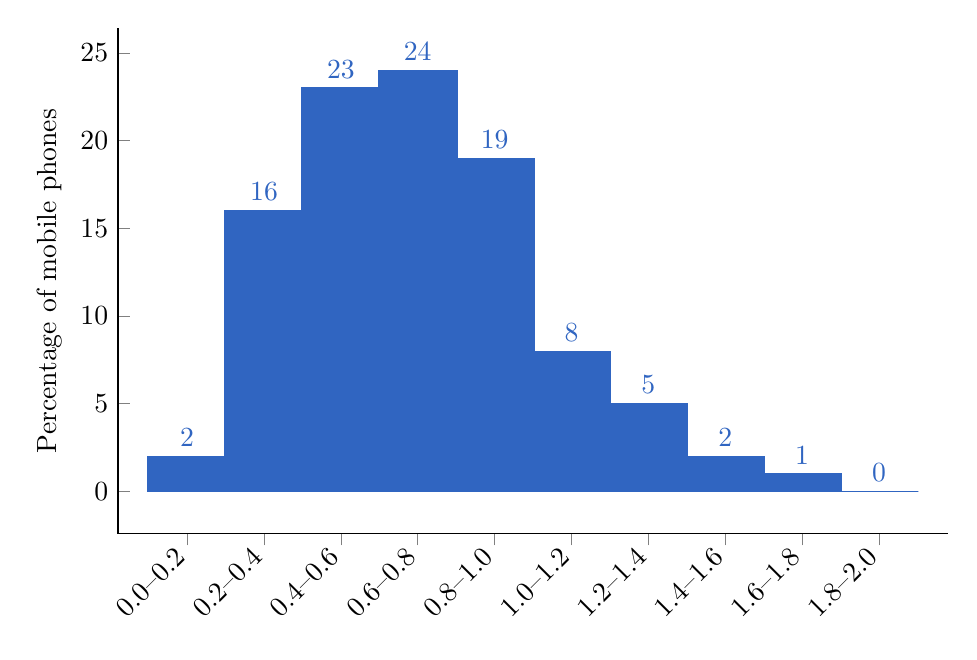
\begin{tikzpicture}
\begin{axis}[
        ybar=-1cm,
        axis x line*=bottom,
        axis y line*=left,
         bar width=1cm,
        height=8cm, width=\textwidth,
        ylabel={Percentage of mobile phones},
        symbolic x coords={0.0--0.2,0.2--0.4,0.4--0.6,0.6--0.8,0.8--1.0,1.0--1.2,1.2--1.4,1.4--1.6,1.6--1.8,1.8--2.0},
        x tick label style={rotate=45, anchor=east, align=left},
        nodes near coords,
        nodes near coords align={vertical}      
        ]
        \addplot[hous,fill]  coordinates {(0.0--0.2,2)};
        \addplot[hous,fill]  coordinates {(0.2--0.4,16)};
        \addplot[hous,fill]  coordinates {(0.4--0.6,23)};
        \addplot[hous,fill]  coordinates {(0.6--0.8,24)};
        \addplot[hous,fill]  coordinates {(0.8--1.0,19)};
        \addplot[hous,fill]  coordinates {(1.0--1.2,8)};
        \addplot[hous,fill]  coordinates {(1.2--1.4,5)};
        \addplot[hous,fill]  coordinates {(1.4--1.6,2)};
        \addplot[hous,fill]  coordinates {(1.6--1.8,1)};
        \addplot[hous,fill]  coordinates {(1.8--2.0,0)};
    \end{axis}
\end{tikzpicture}
todo: xlabel, zeggen dat bovengrens niet inbegrepen is en titel geven.


The $P^{max}_{Tx}$ is for LTE and UMTS 23 Dbm \cite{J11_maxTpxUE, J10_RDP}.

%todo: beslis of je mobile device of UE gaat gebruiken.
To predict the effective transmitted power by the \gls{UE}, the folowing equation is used:

\begin{equation}
P_{Tx} = P_{sens} + PL
\label{eq:ptx}
\end{equation}

\subsubsection{Converting uplink electromagnetic exposure to $SAR^{wb}_{10g}$}
Just like the \gls{DL} radiation expects formula \ref{eq:overallSARwb} the \gls{UL} radiation to be expressed as $SAR^{wb}_{10g}$.
Therefore, the conversion factor from \cite{J22_plets2015joint} for WiFi is reused as explained in \ref{sub:convertDLtosarwb}.

\begin{equation} 
SAR^{wb,ul}_{10g} \left(\frac{W}{kg}\right) = 0.0070 \left(\frac{W/kg}{W}\right) * P_{tx} (W)
\label{eq:solve}
\end{equation}



\subsection{Defining an antenna}
\label{sub:definingAntenna}
A microstrip patch antenna is chosen because it allowes easy production but more important it has a low weight and has a thin profile causing it to be very aerodynamic which is usefull when attaching it to an \gls{UABS} \cite{J13_microstripadvantages}.

The dimensions of the antenna depend on the frequency it is operating and the characteristics of the used substrate.
The antennas will be radiationg at a center frequency $f_0$ of 2.6Ghz. A substrate with a higher dielectric constant and low height reduces the dimentions of the antenna
and a lower dielectric constant with a high height improves antenna performance. The used substrate will therefore be glass with a dielectric constant of 4.4. The height of the antenna is also limited to 2.87 mm in order to keep the antenna light and compact \cite{J14_antennadesign}.
The formulas from \cite{J14_antennadesign} are \cite{J15_antennadesign} applied. 

\begin{table}[h!]
\centering
\begin{tabular}{|l|c|l|}
\hline
 description                & symbol          & value         \\    \hline
 center frequency       & $f_0$           & 2600 Hz       \\ 
 dielectric constant    & $\epsilon_r$    & 4.4         \\ 
 heigt of the substrate & $h$             & 0.00287m    \\ \hline
\end{tabular}
\caption{Overview of configuration parameters}
\end{table}

\begin{equation} 
W = \frac{c}{2*f*\sqrt{\frac{\epsilon_r+1}{2}}}
\end{equation}
Which C the speed of light, $f$ being the center frequency of 2600 Hz and a dielectric contanst of $\epsilon_r$ = 4.4 a width of 3.51 mm is achieved.

$$\epsilon_{reff} = \frac{\epsilon_r+1}{2}+  \frac{\epsilon_r-1}{2} * \left(1+12*\frac{h}{W}\right)^{-\frac{1}{2}}$$
The height of the dielectric is choses to be 2.87mm in order to keep the antenna smal and light\ref{J14_antennadesign}.
$\epsilon_r$ is the permitivity constant of the substrate and depends of the used matieral. In this paper, a substrate like glass is chosen because of the high dielectric constant of $\epsilon_r = 4.4$ compared to other matierals like teflon with only a dielectric constant of $\epsilon_r = 2.2$
This is because larger dielectric decreases the dimentions of the antenna patch \ref{J14_antennadesign} and therefore indirectly also decreases the dimentions of the entire antenna surface which comes in handy for the limited space on drones. When substituting these values, a $\epsilon_{reff}$ of 3.91 is determined.

\begin{equation} 
L_{eff} = \frac{c}{2*f*\sqrt{\epsilon_{reff}}}
\end{equation}
Applying this formula with the known values of above the $L_{eff}$ results in 29.16 mm.

\begin{equation} 
\Delta L = 0.412*h*\frac{(\epsilon_{reff}+0.3)\left(\frac{W}{h}+0.264\right)}{\left(\epsilon_{reff}-0.258\right)\left(\frac{W}{h}+0.8\right)}
\end{equation}
By substituting the values from above, the length extension determines that $\Delta L$ equals 1.3071 mm.

Finally can the lenght of the patch be calculated using the expression: $L = L_{eff} - 2 * \Delta L$
which result in 26.55 mm which result in an antenna like \ref{fig:antennadesign}.

The transmission line model is in fact only applicable for an infinite ground plane but it has been proven that similar results
can be achieved if the groundplane's dimentions are bigger then the patch of approximatly 6 times the height of the dielectric substrate \cite{J14_antennadesign,J15_antennadesign}.

\begin{equation} 
L_{g} = 6 * h + L
\end{equation}
\begin{equation} 
W_{g} = 6 * h + W
\end{equation}

Therefore should the lengt of the groundplane $L_{g}$ be at least 0.0438m and a width of $W_{g}$ 0.0524m.


\begin{figure}[h!]
  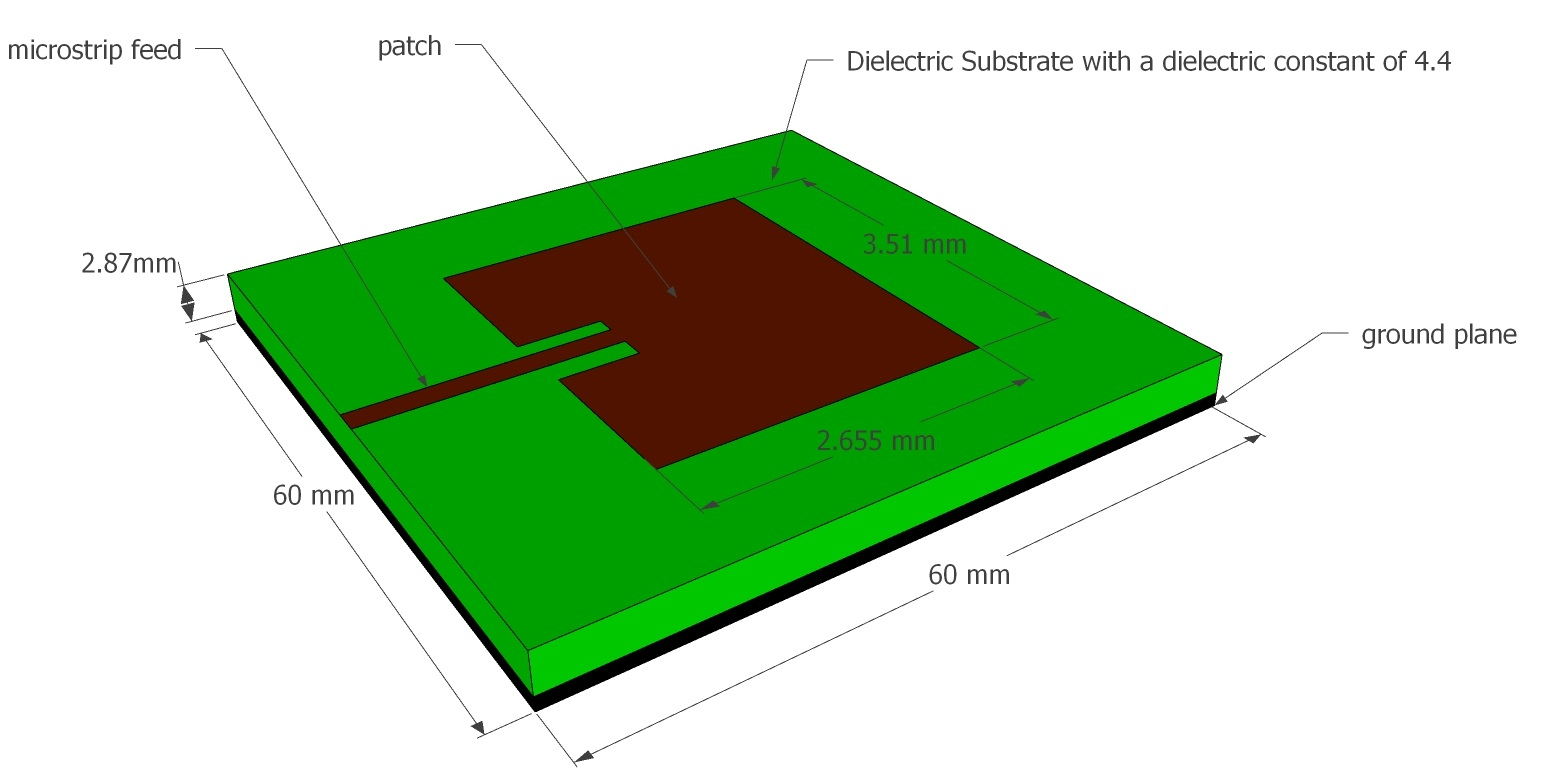
\includegraphics[width=\textwidth]{../images/MicrostripAntenna.jpg}
  \caption{Design of the microstrip patch antenna.}
  \label{fig:antennadesign}
\end{figure}

\subsection{Radiation pattern}
Mathlab is able to generate the radiation pattern for the this microstrip patch antenna.
The code in  \ref{c:mathlabradpattern} starts with defining the dielectric substrate which will be glass with a dielectric constant
of 4.4 and a height of 0.00287m. Thereofter is de microstrip patch antenna generated with the width and lenght being the dimensions
of the radiation patch and the GroundPlaneLength and GroundPlaneLength the dimensions of the groundplane and dielectric substrate.
The FeedOffset is the releative offset from the center where the radio frequency power is fed to the radiating patch which here wil be
at the edge which is in figure \ref{fig:antennadesign} is indicated with the yellow dot. At last is the dielectric object given to the patchMicrostripInsetfed object.

Generating the pattern is done with the 'pattern' command. The first value is the patchMicrostripInsetfed object followed by the frequency
in wich the antenna will be operating. Optionaly can a azimuth value be parsed like in line 7 and 8 where 90 and 0 stand for relatively the H-plane and E-plane.

\begin{listing}[h!]
\begin{minted}[frame=single,framesep=10pt,xleftmargin=20pt,linenos]{c}
d = dielectric("Name",'glass',"Thickness",0.00287,"EpsilonR",4.4)
p = patchMicrostripInsetfed("Width",0.0351,"Length",0.02655,
    "GroundPlaneLength",0.0438,"GroundPlaneLength",0.O524,
    "FeedOffset",[-0.021885 0],"Substrate", d)

pattern(p,2.6e9, "CoordinateSystem", 'polar', "Normalize",true)
pattern(p,2.6e9, 90, "CoordinateSystem", 'polar', "Normalize",true)
pattern(p,2.6e9, 0, "CoordinateSystem", 'polar', "Normalize",true)
\end{minted}
\caption{Mathlab code to generate radiation pattern for a microstrip patch antenna}
\label{c:mathlabradpattern}
\end{listing}

Running the configuration from \ref{c:mathlabradpattern} will generate the radiation pattern from figure \ref{radpattern2}.
When running the same configuration for a slitly bigger square antenna with an edge of 0.060m, the radiation pattern from \ref{radpattern1} is
achieved. It becomes clear that the radiation pattern from figure \ref{radpattern2} has a higher attenuation in de direction it is not facing compared to
the radiation pattern of figure figure \ref{radpattern1}. If it is assumed that drones fly lower then users are possitioned in some buildings, the pattern of \ref{radpattern2}
would be a better approach. However, for the continuation in this master dissertation, the radiation pattern from figure \ref{radpattern2} is assumed since the antenna is the smallest
and therefore more suitable to attach to the limited space available under the drone. A datasheet of the exact values from both radiation patterns can be
found in appendix \ref{ch:radpattern}.

\begin{figure}[!htb]
\minipage{0.32\textwidth}
  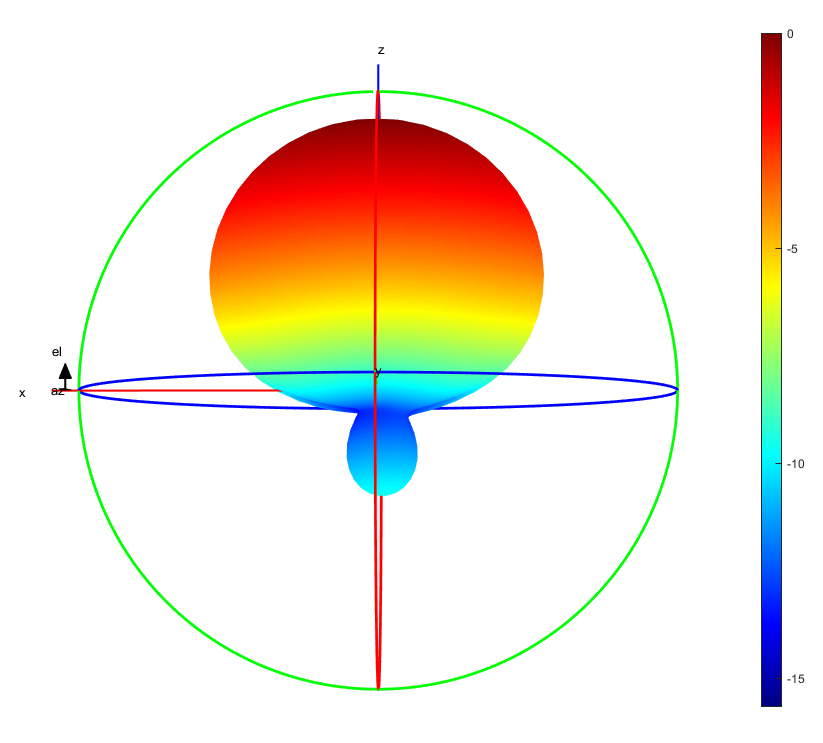
\includegraphics[width=\linewidth]{../images/pattern2/pattern.png}
\endminipage\hfill
\minipage{0.32\textwidth}
  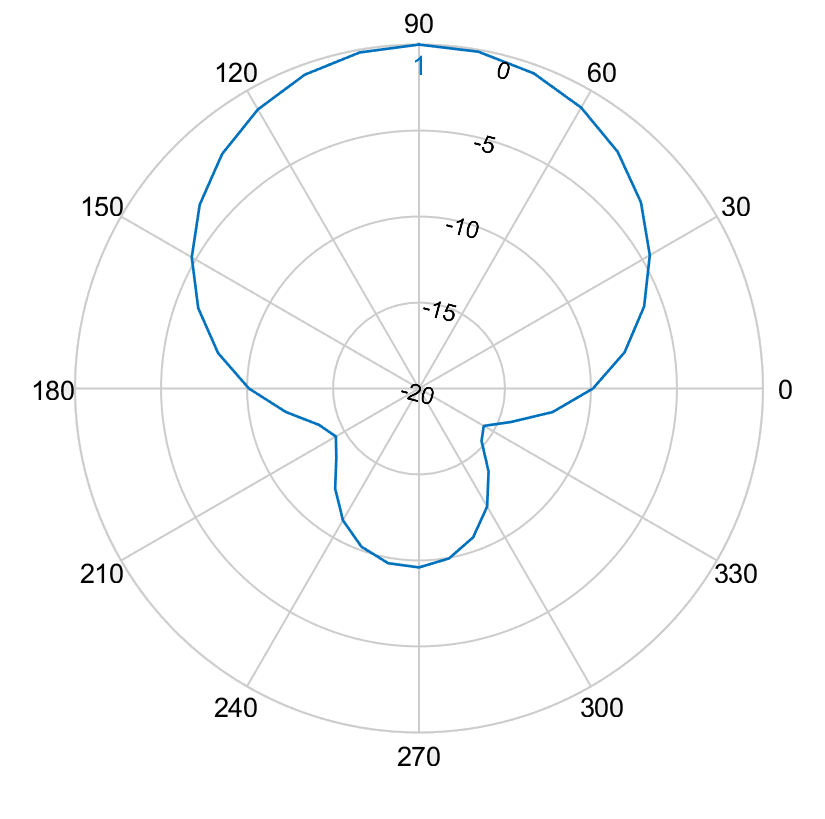
\includegraphics[width=\linewidth]{../images/pattern2/ep.png} 
\endminipage\hfill
\minipage{0.32\textwidth}%
  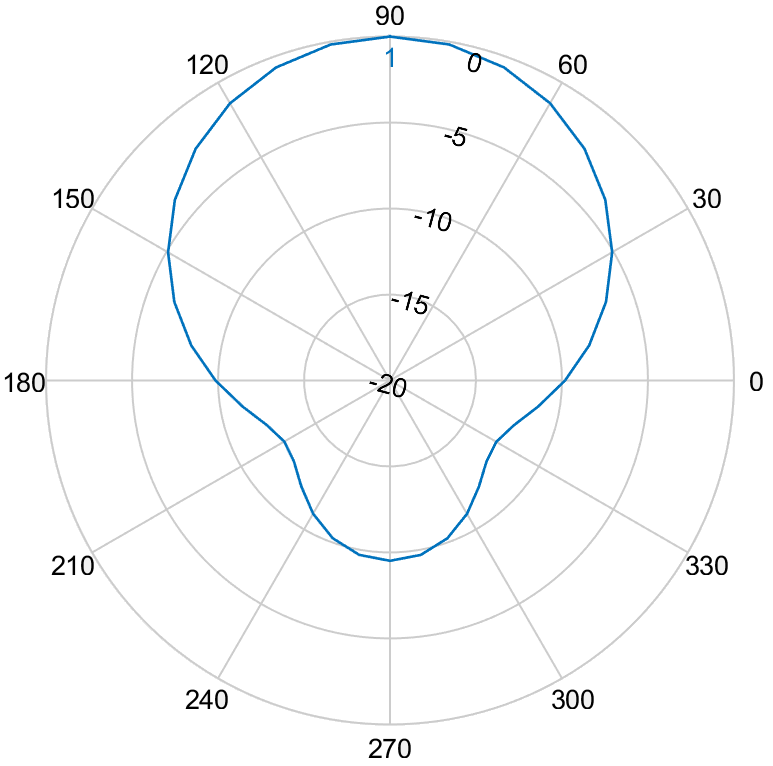
\includegraphics[width=\linewidth]{../images/pattern2/hp.png}
\endminipage
  \caption{Radiation pattern 1: 3D model of the entire pattern on the left with the configuration as discribed above. In the middel a 2D radiation pattern of the E-plane and at the right a 2D model of the H-plane.}
  \label{radpattern2}
\end{figure}

\begin{figure}[!htb]
\minipage{0.32\textwidth}
  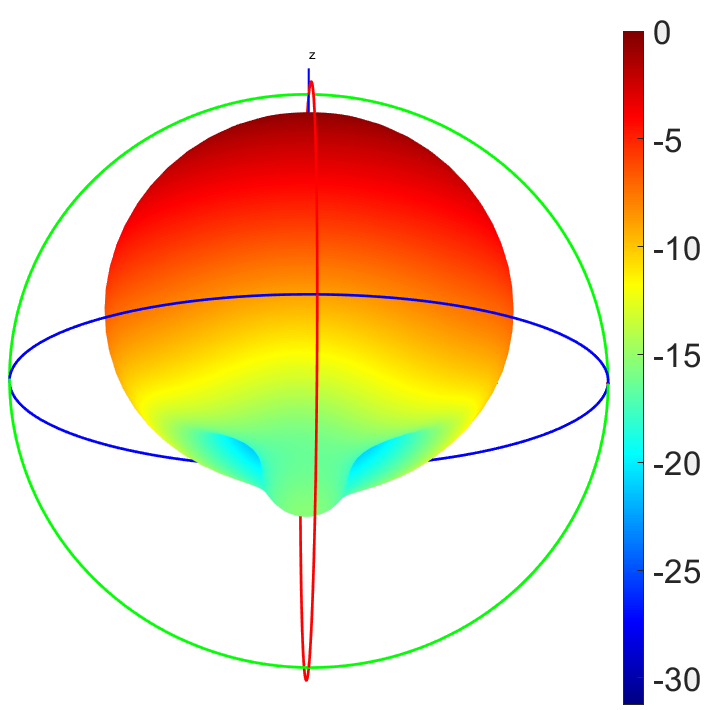
\includegraphics[width=\linewidth]{../images/pattern1/radiationPattern3D.png}
\endminipage\hfill
\minipage{0.32\textwidth}
  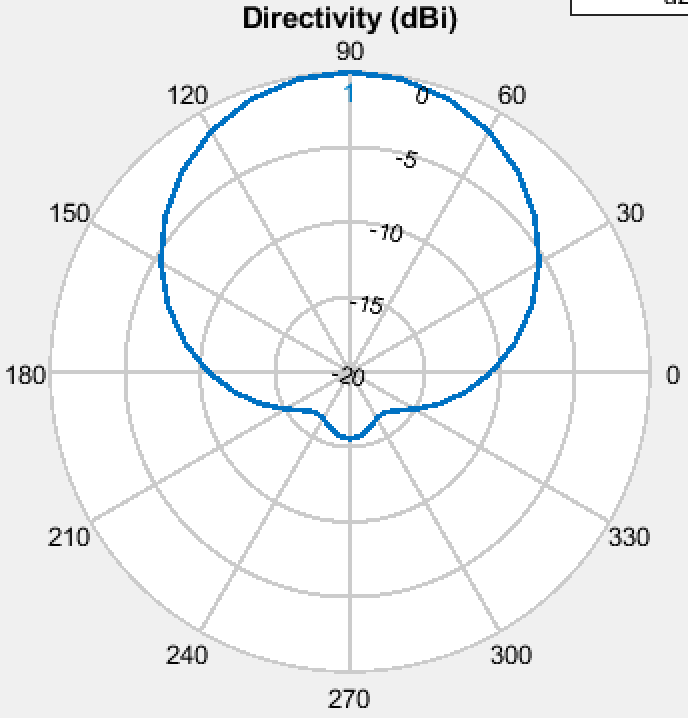
\includegraphics[width=\linewidth]{../images/pattern1/ep.png} 
\endminipage\hfill
\minipage{0.32\textwidth}%
  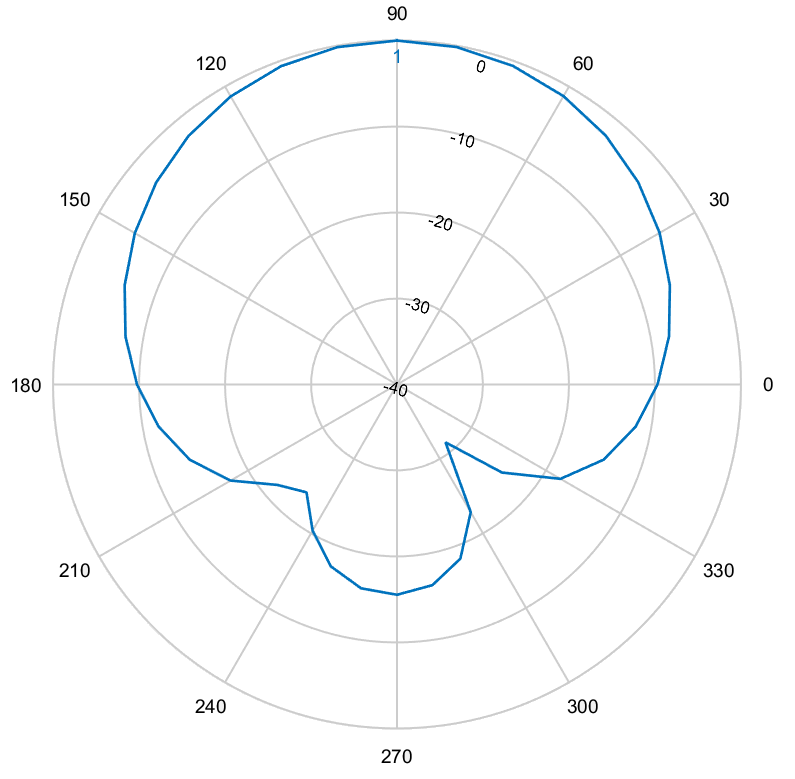
\includegraphics[width=\linewidth]{../images/pattern1/hp.png}
\endminipage
  \caption{Radiation pattern 2: Generated with a groundplane of 0.06m by 0.06m. On the left is the 3D model of the entire pattern plotted. In the middel a 2D radiation pattern of the E-plane and at the right a 2D model of the H-plane.}
 \label{radpattern1}
\end{figure}

\section{Optimizing the network}
The network as originally defined in the deployment tool tried to minimize power consumption by connecting the user to a basestations which
experienced the lowest path loss. A second optimization strategy is introduced, based on the fitness function described in \cite{J1}.

\begin{equation} 
f = w * \left(1 - \frac{E_m}{E_{max}}\right) + (1 - w)*\left(1 - \frac{P}{P_{max}}\right) * 100
\label{eq:fitnessfunction}
\end{equation}

Forumla \ref{eq:fitnessfunction} retuns a fitness value. Users are connected to different \gls{UABS}s and each time the fitness value is 
calculated. The user will eventually be connected to the drone which resulted in the highest fitness value. This process is repeated for each user.
$w$ is the importance factor of electromagnetic exposure ranging from 0 to 1 with boundaries included. A $w$ set to zero means that electromagnetic 
exposure is not important and therefore be called an power consumption optimized network. Likewise, a $w$ set to one will be called an exposure optimized 
network. $P_max$ is the power consumption if all \gls{UABS}s are active and would be radiating at the highest possible level and $P$ the used power by the current network. 
This will be the power required for the flying drones themselves and there antenae.
$E_m$ will be the exposure for the current designed network and $E_{max}$ the electromagnetic exposure when all antenae are at their highest power level.

The weighted average $E_m$ can be found by inserting the median and 95 percentile from all exposures into formula \ref{eq:em}. Since the location of all users in 
the deployment tool are known, it is sufficient to calculate exposure only in those possitions. 

\begin{equation} 
E_m = \frac{w_1 * E_{50} + w_2 * E_{95}}{w_1 + w_2}
\label{eq:em}
\end{equation}

$w_1$ and $w_2$ in \ref{eq:em} being the weighting factors. Not only the median exposure is important but also limiting higher exposure is important. 
Just like \cite{J1} is with that reason $w_1$ and $w_2$ chosen to both have an equal importance of 50 \%.
\textcolor{red}{todo: in J1 is dit gedetailleerder uitgeschreven. Mogelijk om hier wat extra over te schrijven.}


\section{Implementation}

\subsection{Network planning}

TODO
Thereafter, all inactive users are deleted and only the x best bs are kept with x equal to facilityCapacity.
Eventually, exposure is one last time calulcated and objects are initilized with the correct exposure values.

\subsection{Implementation of the radiation pattern}
The deployment tool originally only supported EIRP antennas. The tool thus has been exteded and is fully configurable allowing any possible antenna in any possible 
orientation using the XML-file describing the femtocell. The configuration descripted in this file applies to all \gls{UABS}s. 

The orientation is done using two values called 'downtilt' and 'north offset'. The first value
defines the downtilt angle under wich the antenna is pointing. An angle of 0 degrees is perfectly horizontal and pointing straight to the ground is done with an angle of \ang{90}.
This parameter only supports postive values ranging from zero to 360 (upper boundary not included). An antenna pointing to the sky would therefore require a value of \ang{270}.
The second value, the north offset, difines the azimuth orientation of the drone. The value given to this parameter indicates the offset between the north
and the horizontal direction the antenna should be pointing. The value should once again range from \ang{0} to \ang{360} with the upper boundary not included. The
angle is calculated in counter clock wise orientation. For instance, a north offset of \ang{270} will let the \gls{UABS} point to the east.  

Thereafter, the normalized radiation pattern is supplied to the tool. The actual pattern is three dimensional. To simplefy this,
slices perpendicular to the az-axis are extracted. These are indicated at figure \ref{fig:slicesOfPattern} with azimuth cut. whith
an angle of of \ang{90}, four slices are achieved, easch consisting out of elevation cuts. The intersection of an elevation and azimuth plane 
corresponds with a certain attenuation which is fed to the tool. Figure \ref{fig:slicesOfPattern} show only 3 elevation planes. The radiation pattern used in the tool 
has an attenuation every \ang{10}. In other words, a slice consist of 19 values raning from \ang{0} to \ang{180} (boundaries included).

\begin{figure}[H]
  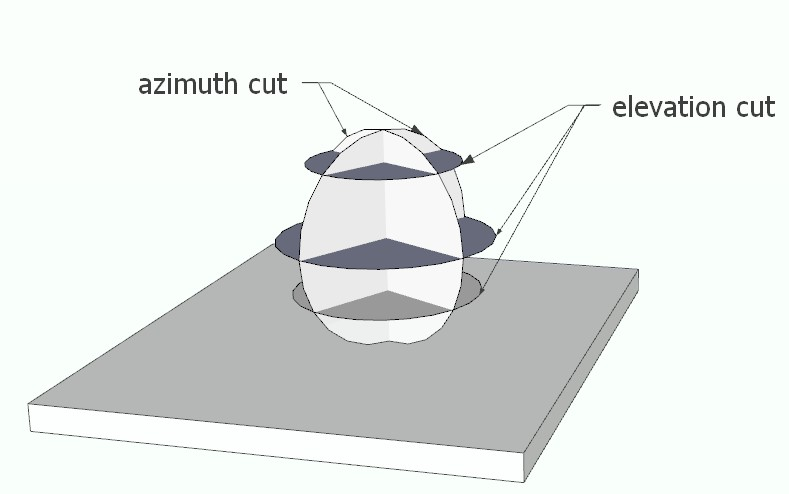
\includegraphics[width=\textwidth]{../images/3Dimages/slicesOfPattern.jpg}
  \caption{Schematic example of slices in a radiation pattern.}
  \label{fig:slicesOfPattern}
\end{figure}
TODO: more slices and elevations. the more slices, the higher the precision. Hoe ondersteund?

When the attenuation of a certain user to that \gls{UABS} needs to be calculated, the angle needs to be calculated
TODO: schrijf hierover.

The change is very little that the angle for which the attenation is requested is known. The attenuation should therefore be esitmated
using bilinear interpollation.

\begin{figure}[H]
\centering
  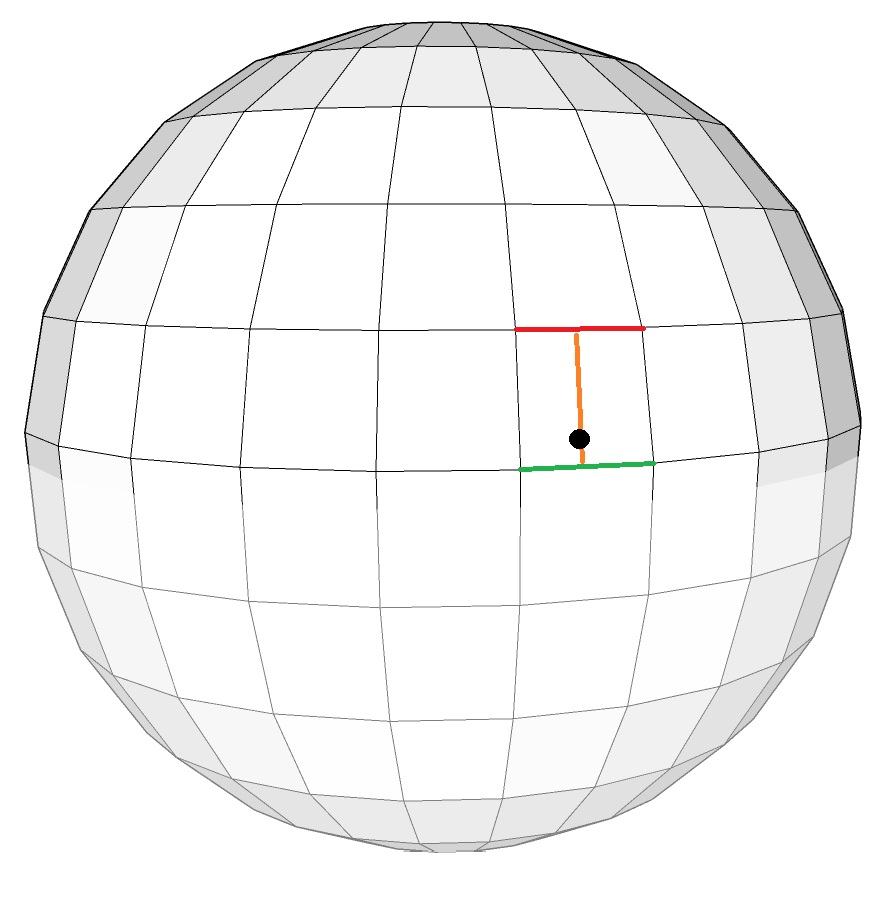
\includegraphics[width=\textwidth/2]{../images/3Dimages/globe.jpg}
  \caption{Schematic example of how bilinear interpollation works.}
  \label{fig:globe}
\end{figure}

\subsection{Performance improvement}
\subsubsection{Calculating pathloss}
The pathloss is required for several formulas. For instance, each user decides whether a \gls{UABS} is feasable based 
the pathloss but also the calculations for the downlink electromagnetic 
exposure require this value to be known. The formulas for the whole body $SAR_{10g}$ require not only the pathloss between the user
and all \gls{UABS}s but even the pathloss between users themselves. These pathloss calculations are based and the Walfisch-Ikegami 
Model and makes a distiction between line-of-sight and non-line-of-sight situations causing a high computational load. The caculation between two points stands completly free from
any other calculation between any other point and is therefore a suitable candidate to be multithreaded. The deployment tool creates two thread pools.
The first pool creates a thread for each user where each thread calculates the pathloss between the user assigned to him and all possible \gls{UABS}s causing a time complexity of $n^2$.
Each user stores all pathlosses between himself and any other \gls{UABS} and result therefore in a total space complexity of $n^2$.
When all users are finished, the pool is shut down and a second one is created for the same calculations but between users.
The pool will, just like the previous, create threads for each user but has an important difference.
When a certain user calculates the pathloss to another user, this pathloss also applies for the other direction. The tool saves time by calculating the pathloss only 
once and stores the pathloss with both users. It is therefore sufficient that a given user only calculates pathlosses to users left of him, since the other will 
be calculated by the users right to him. This results in a time complexity of only $n(\frac{n}{2})$. When the last user finishes his thread, all users know the pathloss to all other users causing 
a space complexity of $n(n-1)$.
% eventueel nog over concurrent hashmap

\subsubsection{Limiting antenna searching}
The user needs to be connected to the 'best' basestation. To indentify this best \gls{UABS}, the user should be connected 
to each basestation and the fitness value \ref{eq:fitnessfunction} of the network should be evaluated. The connection which resulted in the best fitness function
will be added in the solution. This process is repeaded for each user but can further be improved. A user will likly be connected to either 
\gls{UABS} directly above him or to a \gls{UABS} in the direct neighbourhood. Time complexity can thus be improved by not considering drones 
outside a certain radius.
An ideal datastructure for neighbourhood-search is a KD-tree. This datastructure is based on a binary tree and optimal for objects with 
multiple keys. Objects are thus positioned in K dimensions, each node split the hyperplane over exact one dimension. The dimension that need 
to be splitted depends on the level of the KD-tree where that node is situated.
In this case, the x and y coordinate will be used in a 2D-tree (k=2) like in figure \ref{fig:exampleKDtree}.

\begin{figure}[H]
  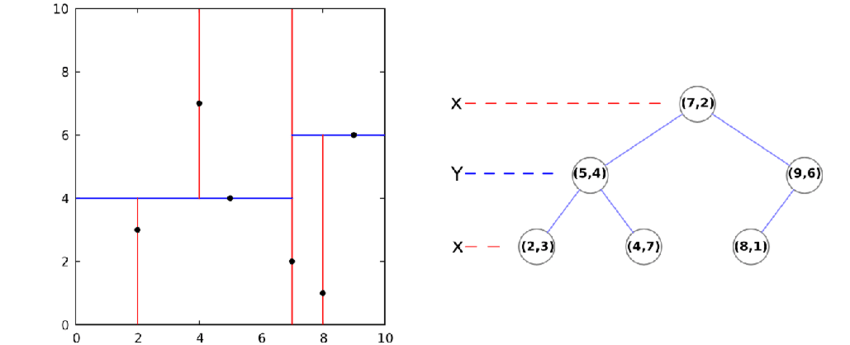
\includegraphics[width=\textwidth]{../images/Example-of-a-2D-k-d-tree.png}
  \caption{Example of a KD-three in two dimensions}
  \label{fig:exampleKDtree}
\end{figure}


Here, is chosen to consider only \gls{UABS}s whithin a radius of half a kilometer. In a scenario of 500 \gls{UABS}s, 60 possible \gls{UABS}s are verified.
TODO: schrijf ook voor 200 users.
